\chapter{Introduction}
\label{cha:introduction}

% dramatic entry
Aggressive behavior has potential beneficial and harmful consequences for the aggressor.
While aggression caries a serious risk of bodily harm for the aggressor, it also has the potential to increase access to resources and higher social status.
The nature and cause of such behavior has always been of interest to social and biological focused researchers and much scientific effort has been spent to investigate the various different facets of this complex behavior.
While previous research has been focused on environmental as well as biological causes of aggressive behavior, here I will solely focus on potential biological mechanisms of human aggression.
Specifically I will investigate potential genetic causes of human aggressive behavior via a variety of different statistical methods.

The first chapter of this thesis will review the existing literature in regards to the definition and forms of aggression, as well as evolutionary theories and known genetic risk factors associated with this complex behavior.
Subsequently, I will give an overview of the statistical methods used within this thesis.
Chapter 3 describes my investigation of over $17,662$ twin pairs to examine the longitudinal heritability of childhood aggression.
The next chapter describes the exploration of specific molecular genetic markers associated with risk taking and aggression in $152,247$ unrelated individuals.
Afterwards, in chapter 5, I will examine the genetic overlap as well as investigate potential causal relationships between psychiatric disorders and aggressive behavior.
Chapter 6 will outline a newly-developed method to test for distributional differences of rare variants.
Finally, I will discuss my findings in detail and outline future research directions.

\section{Definition of Aggression}
\label{sec:overview_of_reseach_in_aggression}

One can define human aggression as a behavior intended to cause physical or emotional harm to others~\cite{Anderson2002}.
However, this definition is rather incomplete since it is also important to consider the unwilling participation of the victim as well.
Indeed, behaviors in which the target does not intend to avoid the aggressive behavior, such as in sexual masochism~\cite{Berkowitz1993,Baumeister1989,Baron2007,Geen2001}, should not be considered  aggressive acts.
Thus the motivation of the victim to avoid such harm plays an important role in the definition of aggression.  
Therefore I will use the following working definition:
\begin{mydef}[Aggression]\label{def:aggression}
	`Aggression is the delivery of an aversive stimulus from one person to another, with intent to harm and with an expectation of causing such harm, when the other person is motivated to escape or avoid the stimulus'~\cite{Geen2001}
\end{mydef}

This definition includes a wide spectrum of violent and nonviolent actions.
Therefore it necessary to specify the broader dimension of aggressive behavior.

\subsection{Forms of Aggression}
\label{sub:forms_of_aggression}

One can separate aggressive behavior into \textit{affective aggression} and \textit{instrumental aggression}.
While \textit{affective aggression} is characterized as emotional, impulsive, thoughtless, and unplanned behavior, \textit{instrumental aggression} is defined as a planned and proactive behavior to obtain a certain higher goal~\cite{Berkowitz1993,Geen2001}.
This distinction has been extended by a number of similar concepts, such as \textit{reactive/proactive} and \textit{offensive/defensive} aggression.
While these terms have slightly different meaning, depending on situation and field of research, the general concept remains similar~\cite{Geen2001, Blanchard2005b}.
In psychology, for example, the terms \textit{affective aggression} and \textit{instrumental aggression} have been established, but more recently authors have used the terms \textit{reactive} and \textit{proactive} aggression~\cite{Geen2001}.
Thus aggressive action in response to a provocation, such as in self-defence and in anger, is \textit{reactive aggression} while planned, unprovoked aggression is called \textit{proactive}.

However, despite the differences in terminology, it is important to emphasise the strong negative emotional state of \textit{affective/reactive} aggression.
This state, often described as \textit{anger}, launches and guides affective aggression  and is often caused by some form of provocation~\cite{Geen2001}.
Nevertheless, \citet{Frijda1994} suggested that \textit{affective/reactive aggression} is not necessarily impulsive.
In some situations, a delay between provocation and aggressive response is observed. 
In particular, long term grudges, or \textit{hatreds}, are preoccupations which go beyond the initial provocation but remain deeply emotional.
Thus I will use the term \textit{impulsive aggression} to refer to impulsive, emotionally-guided, aggressive behavior.

In contrast, \textit{instrumental/proactive aggression} is characterized by the absence of an emotionally strong goal to cause harm.
For example, the use of gossip and bad-mouthing of a colleague in order to obtain higher chances of receiving a promotion is done in a planned manner with the aim of a higher goal.
However, it is often difficult to distinguish actions into affective and instrumental aggression since both forms are not mutually exclusive.
\citet{Geen2001} gave the example of a mother who uses corporal punishment to modify her child's behavior, while still reacting in anger when observing the undesired child's behavior,
hence mixing a planned aggressive act towards a higher goal with an emotional, angry state.

Both forms of aggression, affective and instrumental, can be either physical or verbal.
While physical aggression in humans is homologous to other animals, verbal aggression, a form of \textit{indirect}, \textit{relational}, and \textit{social}, aggression, is relatively distinct to humans~\cite{Archer2005}.
These verbal behaviors cause harm to others by gossiping, spreading rumors, or excluding other from social groups.
While the terms \textit{indirect}, \textit{relational}, and \textit{social} aggression have been differently conceptualized in the past~\cite{Archer2001}, they are expressed in common behaviors and can be contrasted to physical, \textit{direct}, aggression.
Hence the terms are more similar than distinct and I will therefore proceed to call all them \textit{indirect} aggression in order to distinguish it more from the physical, more direct aggressive behavior~\cite{Archer2005}.

Research in animals has often used a slightly different terminology.
Investigations often have distinguished between \textit{offensive} and \textit{defensive} aggression~\cite{Blanchard2005b}.
Similar to \textit{affective} aggression, \textit{offensive} attacks arise from a response to a threat to the animal's resources, thus are the response to a certain provocation.
These resources could be sexual partners, food, social status, or, in the case of humans, money.
On the other hand, \textit{defensive} aggression is a response to a direct threat to the subject's life, a concept closely related to \textit{instrumental} aggression.
While this distinction might hold in mice and rats, the separation between \textit{offensive} and \textit{defensive} aggression is more blurred in primates, including humans.
For example, humans are known to hunt lions and other predators.
In contrast to non-predators, these animals are, for the most part, not eaten which would suggest a form of defensive aggressive behavior.
However, within most human cultures killing a large predator is seen to enlarge one's social status by showing strength and courage towards the others,
a behavior which is an \textit{offensive} action.

However,~\citet{Blanchard2005b} suggest, while the separation between \textit{offensive/affective}  and \textit{defensive/instrumental} might be blurred in humans, the distinction holds in general.
Indeed, the authors suggest that rather insufficient analysis and not a disconnection between animal and human behavior are responsible for the blurred distinction.
However, \citet{Blanchard2005b} provide little evidence for their claims and one can argue that the complexity of human society makes a comparison between subcategories of aggressive behavior across species especially difficult. 
Nevertheless, animal studies have provided valuable insight into aggressive behavior and I will outline a number of experimental findings in animal studies in later sections.

To conclude, one can distinguish between \textit{affective} and \textit{instrumental} forms of human aggression which can be  either \textit{direct} or \textit{indirect}.
Research in non-humans has often distinguished between \textit{offensive} and \textit{defensive} forms of aggression.
I will next consider evolutionary theories in regards to aggression in humans and animals alike.
I will show that aggressive behavior has a strong evolutionary background and that genes which regulate such behavior are under stabilizing selection.

\section{Evolutionary Theories}
\label{sec:evolutionary_theories}

Historically, research on aggression has been divided into nurture versus nature~\cite{Archer2009}. 
Proponents of the nurture side have argued that aggressive behavior is caused by environmental influences, while supports of the nature side of the discussion supported the idea that differences in the genetic architecture are able to explain considerable individual differences in aggressive behavior.
Today's view is less polarized and acknowledges that both nature and nurture play a crucial part in aggression.
While not disregarding the environmental aspect of aggression I will mostly focus on the genetic and biological mechanisms of aggressive behavior.
In the following section I will outline evolutionary concepts helpful in explaining and understanding individual differences in aggression. 

Evidence for a long history of human aggression can be found in  paleontological findings of broken bones, rips and smashed skulls, unexplainable without the consideration of weaponry force.
Occasional findings of weapon fragments in skeletal rib cages suggest that violence and aggression has been part of the human evolutionary history~\citet{Buss1997}. 
\citet{Buss1997}, one of the founders of evolutionary psychology, suggested that all psychological mechanisms and behavior, including aggression, can be explained by the evolutionary principle of selection.  
These mechanisms are aimed to solve specific adaptive problems.
Hence some variants of those behaviors and psychological mechanisms might solve certain problems better than others, thus improving overall fitness.
This results in the preservation, replication, and spreading of theses variants through a population~\cite{Buss1997}.

\citet{Buss1997} suggested \textit{seven} adaptive problems to which aggressive behavior might be an evolutionary solution.
For example, \textit{co-opt the resources of others}, which can be defined as the use of physical or psychological force to obtain resources held by another individual or group, can give the aggressors significant advantages in terms of survival and reproduction.
These resources could mean food, water, land, or sexual partners.
An example of this can be seen in aggressive behavior of children.
\citet{Campbell1995} noted that aggression among toddlers is often about resources, such as toys, suggesting that this behavioral adaptation is a deeply rooted evolutionary strategy.

Aggression can also be useful in \textit{defending against an attack}.
Since attacking aggressors are a serious threat to valuable resources,
aggression can be an effective strategy in defending against individuals or groups.
Furthermore, it can be also an adaptive strategy to foster a reputation that would deter potential aggressors~\cite{Buss1997},
thus avoiding the potential cost of a physical conflict while defending one's resources.

Another evolutionary benefit of aggression can be found in the social hierarchies in groups.
For example, men who win fights and defeat opponents gain power and status in many societies~\cite{Hill1996}.
The gain in social status can be beneficial in accessing resources and mates~\cite{Archer2009}.
Indeed, hierarchical order in social groups is often established by means of aggressive behavior which enables high-ranked individuals priority access to food and partners~\cite{Lindenfors2011}. 
However, aggression can also result in a decline in status.
\citet{Buss1997} suggested for example that a physical conflict between two professors in a faculty meeting would result in a decline in reputation.
Thus displays of aggression are not acceptable in all social situations or always helpful in achieving a goal.

In the context of reproduction one should consider aggression towards the same-sex separate of male-female aggression.
Aggression towards same-sex individuals is sometimes aimed to reduce their social status and therefore make them less attractive to the other sex~\cite{Buss1990}.
Hence inflicting damage on a rival directly translates to an increased benefit to the aggressor.
In addition to aggression towards same-sex individuals, aggression is also prevalent towards the opposite sex.
For example, aggression can be used to deter a long-term mate from infidelity~\cite{Daly1982}.
However, also here aggression can have negative consequences in the form of retaliation.
A husband might be reluctant to use aggression towards his wife when she is living close to a number of brothers and a powerful father.
Indeed, a study in Madrid, Spain, found that women who had a higher density of genetic kin in and around Madrid were less likely to be victim of domestic violence~\cite{Figueredo1995}.
Furthermore, expressing aggression towards another individual sheers energy away from other actives, such as hunting and foraging, and also carries a high risk of injury and death~\cite{Packer1995}.  
This increased cost is also reflected in the conflict resolving methods applied across many animals and humans.
For example, two competing male red deer may begin their confrontation by roaring repeatedly.
If this does not resolve the conflict both will walk side-by-side while attempting to make themselves look as large as possible.
Only the last stage involves a physical confrontation, potentially causing severe injuries~\cite{Clutton-Brock1979}.
These behaviors, aimed to resolve conflicts without the use of raw force, demonstrates the large costs of physical aggression.
However, it  also shows that animals and humans alike are able to avoid those costs by threatening the use of physical force.
\citet{Maxson2005} suggested that if the resource holding potential (\acrshort{rhp}), which is defined as the ability to win a physical fight over resources,  as well the resource value (\acrshort{rv}) itself, are the same for both contestants, conflicts will usually escalate.

Negative consequences might also be present when aggression is used to gain a higher social status.
In a study~\cite{Packer1995} on 138 female baboons in the Gombe National Park in Tanzania high-ranking females showed shorter inter-birth intervals as well as higher offspring survival rates.
Thus one would expect higher life-time reproductive success in baboons with overall higher social rank across their lifetime.
However, the authors were not able to associate reproductive success with mean lifetime rank.
\citet{Packer1995} suggested that this inconsistency can be explained by considering that higher ranked females are also more likely to suffer  miscarriages.
These stress-related failures in reproduction can be seen as a counter-force to a potential arms race among female baboons.
Hence the induced aggression by competing for higher social status carries the cost of significant risk of miscarriages.

Therefore, the increase in fitness due to aggressive behavior, either as a direct gain in resources or higher social status, is balanced by large risks, such as injuries, death, and reduced reproduction.
This would indicate that aggression is under stabilizing selection (see figure~\ref{fig:stab}).

\begin{figure}[hp]
	\centering
	\scalebox{0.6}{\tikzstyle{box} = [rectangle, rounded corners, minimum width=3.5cm, minimum height=1cm,text centered, draw=black]
\begin{tikzpicture}
	\draw[line width=6, gray] (-7,0)-- (0,0) --(7,0);
	\draw[gray, fill=gray] (-1,-2)-- (0,0) --(1,-2) --(-1,-2);

	%Cost
	\node (injury) [box, fill=red!80] at (-5,0.6)  {Reproductive Cost};
	\node (grooming) [box, fill=red!70, above of=injury] {Foraging};
	\node (repo) [box, fill=red!60, above of=grooming] {Parental care};
	\node (foraging) [box, fill=red!50, above of=repo] {Grooming};
	\node (parCare) [box, fill=red!40, above of=foraging] {Injury risk};

	%Benefit
	\node (mat) [box, fill=green!80] at (5,0.6)  {Mating priority};
	\node (res) [box, fill=green!70, above of=mat] {Resource access};
	\node (def) [box, fill=green!60, above of=res] {Predator defense};
	\node (surv) [box, fill=green!50, above of=def] {Survival};
	\node (dom) [box, fill=green!40, above of=surv] {Social Dominance};

\end{tikzpicture}
}
  \caption[Stabilizing Selection of Aggressive Behavior]{Stabilizing selection of aggressive behavior (as in~\citet{Anholt2012}).
  The benefit of aggressive behavior is countered by its cost, thus maintaining a stable level of aggressive behavior within the population}\label{fig:stab}
\end{figure}

Furthermore, same-sex and male-female aggression is not equally balanced among the two sexes and nearly all mammals display sex differences in the expression of aggression, both
qualitative, the type of aggression, as well as quantitative, the amount of aggression.
In general males are more likely to exhibit physical aggression than female.
These sex differences have been discussed in the context of \acrfull{sst}~\cite{Archer2004,Anderson2002,Archer2009}. 
Sexual selection is concerned with how a member of one sex chooses another individual from the other sex, as well as the competition between members of the sex over access to the other~\cite{Darwin1859}.
In most mammals the more competitive sex is the male~\cite{Archer2009}. 
\citet{Trivers1972} suggested that these sex differences can be explained by the limited parental investment by males in many species.
Parental investment is the amount of resources a parent invests into his or her offspring to increase its survival and reproduction~\cite{Archer2009}.
The theory was first suggested by~\citet{0198504403} and proposes that a male can minimize his parental investment in favor in producing a greater number of offspring.
In contrast, many female mammals have a large obligatory parental investment, such as gestation and delivery.
This greater parental investment makes it more important to remain alive in order to raise the offspring,
\citet{Campbell1999} suggested that this discrepancy resulted in more risk-averse behaviors in female.
This would further predict that while direct aggression is quantitatively imbalanced between the sexes, indirect aggression is expressed in both males and females to an equal level due to its lower cost.
Indeed, multiple studies have found no sex differences in indirect aggressive behavior~\cite{NoelCard2008}.
Hence sexual selection can be used to explain sex differences in humans and animals alike.

The above outlined cross-species and evolutionary history of aggressive behavior suggests that inherited biological factors play a key role.
I have shown that aggression, while having large benefits for the aggressor, also caries significant drawbacks.
In the following section I will outline specific genetic aspects associated with aggression.


\section{Biological Mechanisms}
\label{sec:biological_mechanisms}

As outlined in Section~\ref{sec:evolutionary_theories}, aggressive behavior is present in a number of species which indicates that this particular behavior is, from an evolutionary view, relatively old.
However, most findings in regards to the genetics of aggressive behavior comes from animal studies due to the ethical considerations of experimental studies in humans.
Hence previous research has made use of comparative genetics to gain insight into the genetic mechanisms of human aggression.
Comparative genetics is the use and analysis of genomic information across species to identify and relate genes with phenotypes~\cite{Maxson2003}.
A cross species perspective enables one to examine overlapping genes which might affect a particular behavior.
This not only allows one to identify genes involved in aggression across species but also enables consideration of gene-environment interactions.

\subsection{Neurobiology of Aggression}
\label{sub:neurobiology_of_aggression}

Numerious studies have investigated the neurobiology of human aggression and violence.
Within this section I will describe the neuroanatomy, functional connectivity, neurochemistry of aggression. 
Specically, I will focus on the involvement of the amygdala and amygdala-frontal circuitry. 
Furthermore, I will describe the involvement of the serotonergic system on aggressive behavior as well as the contribution of steriod hormones, such as cortisol and testosterone.

\subsubsection{Neuroanatomy and Functional Conectivity}
\label{ssub:neuroanatomy_and_functional_conectivity}

The amygdala is a medial temperoal lobe structure which is involved in a number of crucial tasks, such as the processing of a sensory and motivatioanlly salient stimuli as well as their tranmission to cotrical and subcortical areas.
Thus the amygdala is crucial for emotional related learning and memory formation~\cite{Salzman2010}.
Crucially, the amygdala is composed of 3 main nuclear complexes.
The basolateral, central and cortical area.
The role of both the basolateral and central complex are well understood, while little is known about the cortical area of the amygdala.
While the basolateral complex is primarily involved in the processing of sensory information within the amygdala, the central complex is considered the main output component due to its interconnectivness to various subcortical and brain stem areas~\cite{Sah2003}.

Interestingly, structural imaging studies have repeatedly found a negative correlation between the size of the amygdala and aggressive behavior.
In a sample of 20 nonclinical female participants right and left amygdala volumns were smaller in those who scored higher on measurements of lifetime aggression.
This effect seems to be specificly related to aggressive behavior since measurements of general pschopathology, trait anxiety and state depression were uncorrelated with amygdala volumns~\cite{Matthies2012}.
Similar results were shown in a longitudinal study by~\citet{Pardini2014} of 56 participants who were psychometicly assessed at three seperate time points: Childhood, at the age of 26, as well as at age 30.
The authors showed that amygdala volumns measured at age 26 were negatively correlated with childhood aggression scores.
In another study of 566 children~\citet{Thijssen2015} found significant samller amygdala in children who scored higher on parent indicated levels of aggression.

In order to further understand the amygdala and the role it plays within aggressive behavior, multiple studies have started to differentiate between its anatomical structures.
In a sample of 41 psychiatric patients~\citet{Gopal2013} showed that the left cental amygdala was negatively correlated with lifetime history of aggressive behavior.
Interestingly, this particular study found that both left and right basolateral amygdala complex was positivly associated with impulsivity.
Thus suggesting an anatomical and hemisphrical specialization of the amygdala in regards to aggression.

However, anatomical and structural associations does not necessaryly indicate functional differences.
A study by~\citet{New2009} showed differences in baseline amygdala activity as well as in response to provocations between patients ($N=38$) affected by intermittent explosive disorder (IED) and controls ($N=36$).
The authors used 18-fluoro-deoxyglucose positron emission temography (FDG-PET) as well an laboratry aggression task.
At baseline the IED group exhibited hypo-metabolic rate compared to controls, while in a provocated state amygdala activity increased in patients and decreased in controls.
Thus suggesting that amygdala activity is more unstable in patients with pathelogical aggressive behavior.

Differences in amygdala acitivities have also been observed in functional magnetic resonance imaging (fMRI) studies.
\citet{Coccaro2007} demonstrated enhanced amygdala activies in response to threatening facial expressions in IED patients (N=10) compared to controls (N=10).
Interestingly~\citet{Bobes2013} found hyper-active amygdala responses to fearful and neutral faces in a group of violent men (N=25) compared to controls (N=29). 
Thus indicating that more aggressive individual exhibit stronger amygdala response to faces in general.

In addition to the amygdala, the limbic prefronatal conrtex (PFC), which includes the orbitofrontal cortex (OFC) and the anterior cingulate cortex (ACC), have been implicated in aggressive behavior.
While the OFC is generally seen as integrating sensory and perceptual information to evaluate the motivational value of stimuli, the ACC is more associated with actions and responses~\cite{Rudebeck2014,Walton2007}.

Indeed various studies have shown negative correlations between ACC and OFC volumns.
A study by~\citet{Ameis2014} of 297 healthy children between the ages of 6 and 18 suggests that volumns of both left OFC and ACC were lower in those who scored higher on externalizing behavior.
Interestingly, the studies by~\citet{Ducharme2011} and~\citet{Boes2008} confirm an associations between OFC and ACC volumns and children's aggressiveness measurements.
However, both studies show a postive rather than a negative correlations.
Furthermore, the study by~\citet{Thijssen2015} with 566 children was unable to find any significant differences in OFC and ACC volumns.

While there are considerable questions in regards to OFC and ACC volumn differences, variation in amygdala-PFC connectivity are more clear.
~\citet{Coccaro2007} showed that interconnectivity between amygdala and PFC was absent or reduced in patients suffering from IED.
In a stimilar study of 25 schizophrenic patients~\citet{Hoptman2010} demonstrated negative correlations between amygdala-frontal activity and measurements of aggressive behavior.
This effect seems also to be present in non-clincal samples.
For example,~\citet{Fulwiler2012} showed in a sample of 16 healthy male participants that amygdala-OFC connectivity was negatively correlated with measurements of anger. 
Thus there is considerable evidence for a negative associations between aggression and amygdala-frontal connectivity.
However, it remains unclear how amygdala-PFC connectivity is modulated.
In their review~\citet{Rosell2015} suggested the serotonergic system as the most likely candidate.

To summaries, multiple studies have found negative correlations between amygdala volumn and measurements of aggression. 
Similar, some studies have suggested lower OFC and ACC volumns in subjects with higher aggressiveness scores.
However other studies were unable to replicate these size differences.
Furthermore various studies in clincal and non-clincal samples have found lower levels of interconnectivity between amygdala and PFC in subjects who score higher on measurements of aggression.

\subsubsection{Neurochemistry and Pharmacology}
\label{ssub:neurochemistry_and_pharmacology}

The serotonergic system is one of the most well studied neurobiological system in aggression.
One of the first evidence for an involvement of seotonin (5-HT) in aggression came from animal studies.
Specically various 5-HT antagonists reduced aggressive behavior in mice~\cite{Malick1976}.
Furthermore multiple studies have shown lower levels of 5-hydroxyindoleacetic acid (5-HIAA), a major metabolite of 5-HT, in the cerebrospinal fluid (CSF) of patients with personality disorders~\cite{Brown1982,Brown1979}.
In addition, selective serotonin reuptake inhibitor (SSRI), a common used antidepressant, has been shown to reduce aggressive behavior in patients affected with personality disorders~\cite{Zanarini2004,Coccaro1997a}. 

These findings have lead to the use of agents that can moderate central 5-HTergic functions in experimental settings.
For example, a number of studies have used diatry depletion of tryptophan which results in significant lower 5-HT activity~\cite{Williams1999,Carpenter1998}.
Indeed~\citet{Bjork2000} showed that tryptophan depletion increased  aggressiveness in responses to experimental stimuli, while tryptophan enrichment resulted in lower levels of aggression.
However, this negative correlation between tryptophan and aggression was only present in subjects with high levels of baseline aggression, while subjets with low baseline levels showed the reverse effect.
Nevertheless, this effect has not been replicated by all studies.
Indeed mutliple studies only find an increased responses in aggressiveness to experimental stumuli in subjects with low levels of baseline aggression~\cite{Stadler2008,Kotting2013,Kramer2011}

The observed effect of 5-HT on aggressiveness has lead to some studies investigating its involvement in impulse control and emotional processing.
For example~\citet{Passamonti2012} demonstrated, in a randomized control trial of 19 subjects, that tryptophan depletion can significant reduced amygdala-PFC connectivity in responses to angry faces.
Thus demonstrating that 5-HT affects aggressive behavior most likely through the amygdala-PFC neural network.

These experimental findings make it not surprising that experimental disruption of 5-HT receptors have also been shown to have profound effect on aggressive behavior.  
For example, mice whose \textit{5-HT1B} receptor was knocked out demonstrated hyper-aggressive symptoms while those which were treated with \textit{5-HT1A} receptor antagonist displayed reduced levels of aggression~\cite{Saudou1994,Bell1994}.

Also the serotonin transporter (5-HTT) has been subject to investigations.
A polymorphism in \textit{5-HTTLPR} (consitent of a short or long allele)  has been found to result in higher levels of aggressive behavior in  people with depression~\cite{Gonda2011} and intellectual disabilities~\cite{May2010}, while not demonstrating associations in non-affected subjects.
\citet{Anholt2012} suggested that hese associations as an indicator for a gene-environment interactions.
However, given the small sample size of the studies, other possibilities might explain these findings.
For example shared genetic mechanism between depression, intellectual disabilities and aggression, could also explain the increased effect of polymorphism in \textit{5-HTTLPR} on aggressive behavior. 
Nevertheless, the identification of gene-environment interaction within aggressive behavior suggest a complicated underlying genetic architecture.
Interestingly, another polymorphism within the second intron of the \textit{5-HTT} gene has been shown to influence aggressive behavior.
Specically, a \acrfull{vntr} size 10 to 12 within \textit{STin2}~\cite{Aluja2009}. 
This effect seems to be pronounced when the short allele of \textit{5-HTTLPR} and as well as the 12-repeat allele of \textit{5-HTT} are present. 

In addition to receptor and transporter of 5-HT, a well known enzyme, whose major neurochemical subtractes is 5-HT, has been found to be involved in aggression.
Namely monoamine oxidase A (MAOA), whose involvement in aggression was discovered when analysing a large Dutch family~\cite{Brunner1993}.
In particular, male members of this family were known for their aggressive behavior, including arson, attempted rape, and other forms of aggression.
Genomic analysis revealed that individuals had a deficient monoamine oxidase due to a point mutation in the \textit{MAOA} gene, suggesting a causal link between \textit{MAOA} and aggressive behavior.
Interestingly, this causal link has been replicated multiple times in humans~\cite{Huang2004,Manuck2000} as well in mice~\cite{Cases1995} and monkeys~\cite{Newman2005}.

Interestingly, a number of studies have shown gene $\times$ environment interaction effects.
\citet{Caspi2002} showed in a sample of $499$ male children that some children who were maltreated developed anti-social behavior.
This effect seemed to be moderated by a mutation in \textit{MAOA}.
Children with higher expression of \textit{MAOA} were less likely to suffer from anti-social behavior following maltreatment.
These results were later replicated by a number of similar studies~\cite{KimCohen2006}.
However, not all studies were able to replicate these findings.
\citet{Anholt2012} suggested that the failure to replicate can be explained by the low statistical power of some of the studies as well as diversity of the used samples, including sex, age, and ethnicity.
Indeed, other studies have found a more complex picture of \textit{MAOA}-environment interactions.
\citet{Huang2004} for example showed that this gene-environment interaction is male-specific, and~\citet{Weder2009} demonstrated that extreme cases of maltreatment did not result in varying effects of later anti-social behaviors.
Nevertheless, it is still unclear how maltreatment in childhood results in anti-social behavior later in life and how \textit{MAOA} is moderating this effect.
Furthermore, most studies had little statistical power,
thus large scale population data is necessary to confirm this gene-by-environment interaction.

In addition to serotonin, the dopaminergic system has been shown to be involved in aggression.
However, only a few studies have so far been conducted.
\citet{Schluter2013} investigated dopamin storage and synthesis via a PET imaging using \[(18)F\]DOPA in a sample of 21 healthy male adults and participants were given an experimental task to assess aggression.
Interestingly, both dopamin storage and synthesis was negatively associated with aggressive responses.
This stands in contrast to a similar study by~\citet{Buckholtz2010} who demonstrated a positive correlations between presynaptic dopamin release and anti-social behavior in a non-clincal sample of 30 participants. 
\citet{Rosell2015} speculated that the apparent confict between these two studies can be explained by the differences in the two traits measured.

The observation that dopamin might play an important role in the neurobiology of aggressive behavior it should come to no surprise that individual dopamin receptors have been shown to be involved.
For example,~\citet{Hohmann2009} identified an association between a \acrfull{vntr} and externalizing behavior in the dopamine D4 receptor (\textit{DRD4}) gene.
Interestingly, subjects who also had a mutation in the serotonin transporter \textit{SLC6A4}, specifically in the serotonin-transporter-linked polymorphic region (\textit{5-HTTLPR}), showed high levels of aggressive behavior.
This behavior was not present if only one of the two mutations were present.
Hence this is a rare display of a gene-by-gene interaction, also called epistasis~\cite{Anholt2012}, in a behavioral phenotype.

\subsubsection{Steriod Hormones: Testosteron and Cortisol}
\label{ssub:steriod_hormones_testosteron_and_cortisol}

There is considerable evidence that both testosteron as well as cortisol contribute to aggressive behavior.
One of the first studies identifying a relationship between testosteron and aggresion was conducted by~\citet{Dabbes1991}.
The authors showed in a sample of 113 late-adolescent male criminal offenders higher testosteron concentration in those who commited more violent crimes.
Interestingly however, this effect seems to be only present in subjects with low levels of cortisol~\citet{Popma2007}.

\citet{Rosell2015} furthermore suggested that the relationship between testosteron and cortisol might differ depending on sex and whether subjects exhibit clincal psychopathatic traits.
Indeed,~\citet{Kuepper2010} showed that testosteron was only associated with higher levels of aggression in men but not women.
In addition, the moderating effect of cortisol seems to be more complicated than the study by~\citet{Dabbes1991} suggested.
For example,~\citet{Welker2014} showed in a non-clincal sample of 237 participants that correlations between aggression and testosteron was negative in participants with low levels of control concentration, but positive in those with high levels of contrisol.
Thus suggesting a considerable more complicated testosteron-cortisol interaction.

A number of studies have also started to look at the neurobiological mechanisms underlying the effect of control and testosteron on aggression.
Indeed,~\citet{Derntl2009} have shown that amygdala response rate was positivly correlated with testosteron levels in reaction to fearful facial expressions.
Similar~\citet{Hermans2008} demonstrated that amygdala, hypothalamus and brainstem activation was directly related to the ratio of testosteron to corisol in a sample of 12 healthy subjects.
Furthermore,~\citet{VanWingen2010} showed that testosteron is not only active within the amygdala but also plays a central role in the amygdala-PFC circuitry.
Specically, the authors showed in a sample of nonclinical female participants that intransal testosteron administration reduces the functional connectivity between amygdala and left OFC during a facial emotional processing task.

These studies suggest both control and testosteron have a relevant effect on aggressiveness, probably by modulating the interconnectivity between amygdala and PFC during fear or threat responses.

\subsection{Investigative Approaches}
\label{sub:investigation_approaches}

\citet{Maxson2005} proposed three general approaches to investigate the genetic architecture of aggressive behavior.
(1) One can identify genes by mapping their sequence to different forms of aggression (see my own study in Chapter~\ref{cha:assocation_study_in_agggressive_behavior_and_risk_taking}).
(2) Another approach is to alter the genetic code of experimental organisms, such as rats and mice, to test for the effects of different genes on aggression.
(3) Last, one can measure the rate of gene expression within the brain in association with an aggressive phenotype.
Only in recent years options (1) and (3) have been made possible due to progress in the sequencing of human and animal genomes.
Option (2) has the highest scientific validity due to the use of randomized control trials, a method only available in nonhuman animals.
However, one can also add a fourth and fifth category.
Indeed, investigation of DNA methylation in order to uncover the epigenetic mechanisms of aggressive behavior is gaining more traction.
DNA methylation is a biological control mechanism by cells to control gene expression.
While studies on DNA methylation in human aggression have been only recently  conducted~\cite{VanDongen2015a}, this new field of study is potentially promising in investigating the genetic mechanisms of aggression.
Further, while~\citet{Maxson2005} only described molecular methods, one can also make use of twin pairs.
Twin studies make use of the genetic similarity (or dissimilarity) of dizygotic and monozygotic twins, since dizygotic twins, and siblings for that matter, share on average 50\% of their genetic makeup with their brother or sister, while monozygotic twins share 100\%.
This enables one to estimate the genetic contribution of aggressive behavior in humans.
These studies have been a popular method to investigate the genetic contribution of a variety of different phenotypes and I will outline a detailed description of this particular method in Section~\ref{sec:twin_based_studies}. 
Most twin studies have estimated the genetic contribution to aggressive behavior between 50\% and 80\%~\cite{Porsch2016}.
While these estimates give a broad understanding about the importance of genetic factors  to aggression, twin studies are unable to inform about specific genes or genetic markers.

Within the following section I will outline previously uncovered specific genetic associations in human and nonhuman animals alike.
Further I will discuss previous findings in regards to gene-gene and gene-environment interactions.


\subsection{Genetic Associations in Nonhuman Animals}
\label{sub:genetic_associations_in_animals}

Genetic analysis in animals has a number of advantages.
First, one is able to make direct manipulation of the genome in question, and second, one is able to quantify aggressive behavior more easily.
For example, aggression in mice can be measured by counting the number of attacks the animal performs when placed in a situation which involves social confrontation with another mouse.

Furthermore, the knock-out of the non-functional nuclear receptor \textit{NR2E1} has been shown to result in a hyper aggressive state in mice~\cite{Young2002}.
Also a knockout of \textit{NOS1} in mice showed an increased level of aggressive behavior.
Interestingly, this particular knockout not only resulted in a hyper-aggressive state but also in a behavior which can be described as a relentless attack on opponents who had surrendered or showed no interest in a confrontation.
Hence these mice demonstrated a qualitatively different aggressive behavior compared to other mouse knock-outs.
Further, within these animals one could observe clear sex differences.
While male mice showed the above-described hyper aggressive state, female mice showed a reduced aggressive behavior against male invaders~\cite{Gammie1999,Nelson1995}, demonstrating a sex-specific genetic regulator of aggression.

\subsubsection{Gene-Gene Interaction in Nonhuman Animals}
\label{ssub:Gene-Gene_Interaction_in_nonhuman_animals}

In their review,~\citet{Anholt2012} pointed to a number of gene-gene interactions which seem to regulate these single gene effects.
For example, the knockout of \textit{NR2E1} had different effects depending on the genetic background~\cite{Young2002}.
While the mouse models C57BL/6J-frc and B6129F1-frc both displayed increased levels of aggression, C57BL/6J-frc demonstrated significantly more aggressive behavior,
 suggesting that the knock-out resulted in a different effect depending on the genetic background.
Identification of gene-gene interactions in humans, however, remains difficult due to the lack of sufficient sample size in many genome-wide association studies.

\subsection{Genetic Associations in Humans}
\label{sub:genetic_associations_in_humans}

Genetic association studies in humans commonly face difficulties in obtaining large enough sample sizes and therefore lack statistical power.
Indeed, in one of the most comprehensive meta-analyses, no genome-wide significant signal was detected~\citet{Vassos2014}.
However, studies included in this meta-analysis showed a considerable degree of heterogeneity in the phenotype.
Specifically, it included psychiatric as well as population-based samples, hence impairing the authors' ability to detect genome-wide significant signals.
Indeed, in their review of association studies of aggressive behavior,~\citet{Fernandez-Castillo2016} found that most hypothesis-free approaches lacked sample size, assessed often very heterogeneous phenotypes, and did not differentiate between direct and indirect aggression. 
A notable exception is the GWAS by~\citet{Pappa2016a}.
The study is relatively large (N = $18,988$) compared to previous approaches and only included children between early childhood and early adolescents.
Furthermore, aggressive behavior was assessed with well-validated parent-reported questionnaires. 
However, also this study failed to identify any significant SNPs, but gene based analysis suggested an association within \textit{AVPRI1A}.

Thus other studies have focused on only a handful of selected genes to investigate the genetic architecture of human aggression.
For example, Alzheimer patients who are homozygous for the \textit{apolipoprotein E $\epsilon 4$} allele have been reported to express more aggressive behavior~\cite{Craig2004,VanDerFlier2006}.
However, these findings could not be replicated in a study with larger sample size~\cite{Hollingworth2006}.
Also studies on the catechol-O-methyl transferase gene (\textit{COMT}) in schizophrenia have associated a single polymorphism with aggression~\cite{Hirata2013,Calati2011}.
Similar to the findings in mice, a single-gene association study of $1,308$ patients with attention deficit/hyperactivity disorder (ADHD) and a criminal history demonstrated that a single polymorphism in the \textit{NOS-I} gene was associated with aggressive behavior~\cite{Reif2009}.

\section{Genes and the Environment}
\label{sec:gene_environment_interactions}

Many behavioral phenotypes depend on the surrounding environmental conditions (see Figure~\ref{fig:plasticity}).
For example, in threatening situations, one might be prone to exhibit more aggression compared to non-threatening circumstances. 
On the other hand, gene-environment interactions is when the phenotypical expression of one genotype depends on environmental stimuli (see Figure~\ref{fig:gene_env_interaction}).
Interestingly, aggressive behavior is one of the few behavioral phenotypes were previous research has shown gene-environment interactions.

\begin{figure}[!htp]
  \centering
  \begin{subfigure}[t]{0.4\textwidth}
    \centering
    \resizebox{\linewidth}{!}{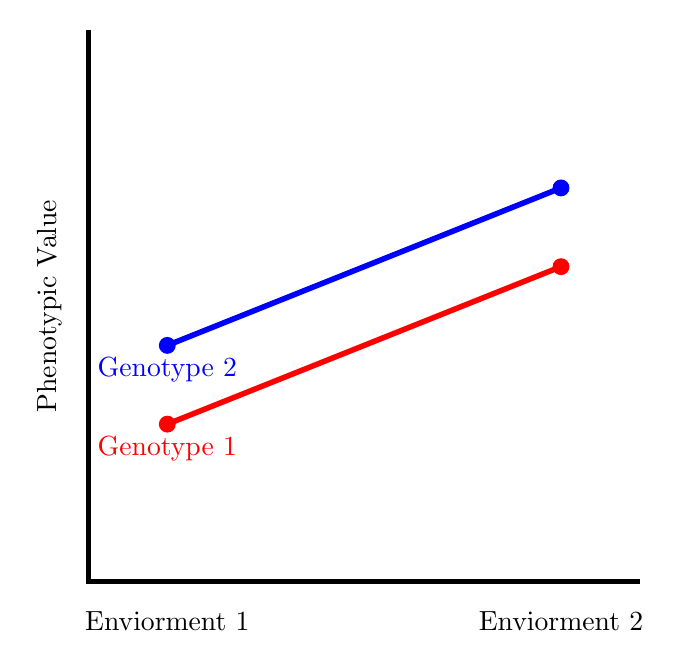
\begin{tikzpicture}
	% axes
	\draw[line width=2, black] (7,0)  -- (0,0) --(0,7);

	% interaction
	\draw[line width=2, red] (1,2) node[below] {Genotype 1}-- (6,4);
	\draw[red, fill=red] (1,2) circle (0.1cm);
	\draw[red, fill=red] (6,4) circle (0.1cm);

	\draw[line width=2, blue] (1,3) node[below] {Genotype 2}-- (6,5);
	\draw[blue, fill=blue] (1,3) circle (0.1cm);
	\draw[blue, fill=blue] (6,5) circle (0.1cm);

	% text
	\node at (1,-0.5) {Enviorment 1};
	\node at (6,-0.5) {Enviorment 2};
	\node[rotate=90] at (-0.5,3.5) {Phenotypic Value};
\end{tikzpicture}
}
    \caption{Phenotypic plasticity}\label{fig:plasticity}
  \end{subfigure}
  \begin{subfigure}[t]{0.4\textwidth}
    \centering
    \resizebox{\linewidth}{!}{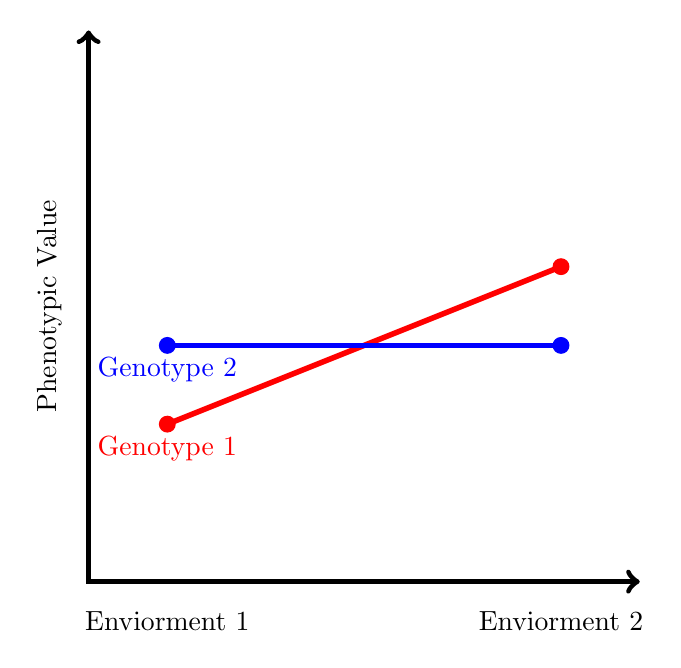
\begin{tikzpicture}
	% axes
	\draw[line width=2, black, <->] (7,0)  -- (0,0) --(0,7);

	% interaction
	\draw[line width=2, red] (1,2) node[below] {Genotype 1}-- (6,4);
	\draw[red, fill=red] (1,2) circle (0.1cm);
	\draw[red, fill=red] (6,4) circle (0.1cm);

	\draw[line width=2, blue] (1,3) node[below] {Genotype 2}-- (6,3);
	\draw[blue, fill=blue] (1,3) circle (0.1cm);
	\draw[blue, fill=blue] (6,3) circle (0.1cm);

	% text
	\node at (1,-0.5) {Enviorment 1};
	\node at (6,-0.5) {Enviorment 2};
	\node[rotate=90] at (-0.5,3.5) {Phenotypic Value};
\end{tikzpicture}
}
    \caption{Gene-by-enviornment interaction}\label{fig:gene_env_interaction}
  \end{subfigure}
  \caption[Gene-Environment Interactions]{Different interactions between genes and the environment. 
    The colors represent different genotypes~\cite{Anholt2012}. 
    (a) Different environments result in the same effect independent of genotype.
    (b) The effect of the environment is genotype-specific}\label{fig:env_interactions}
\end{figure}

\bigskip

In conclusion, I have outlined definitions of aggressive behavior and evolutionary theories and concepts surrounding it.
Further, I have reviewed and described previous research into specific genetic aspects of aggression in human and nonhuman animals alike.
In addition I have shown that previous research has also demonstrated considerable gene-environment interaction within aggression.
In the following chapter I will describe methods used to investigate the genetic architecture of human aggression.
